\section{Implementing Synchronization}\label{sec:impl_sync}
In this section we discuss how we implement the methods of synchronization we discussed in \cref{cha:sync}.
First we summarize what lead us to implementing synchronization the way we did.
Then we will explain how each of the implemented synchronization methods work, and lastly we explain where we use the synchronization in the app.

In \cref{sec:sync_conclusion}, we decided that \ac{NTP} would suit us best.
However due to the complexities of \ac{NTP} we decided to implement \ac{SNTP}, which only considers the latest synchronization to the \ac{NTP}-server, and discards old results.

Since a persistent internet connection is not an ideal requirement for our application we also implemented our own time-synchronization over the local wireless network, made using WiFi Direct.
This method would not synchronize each slave to a global clock, like \ac{NTP} and \ac{SNTP}, but rather synchronize the clock of the slaves to the clock of the master.
However for our application this it not a worry, our goal is to synchronize audio accurately across devices in our network, which does not require each clock to be globally synchronized, only locally.

We decided to implement both of these, that is \ac{SNTP} over the Internet and time-synchronization over WiFi Direct.
In order to determine which is best, we will test them against each-other.\tnwarning{We need to do this}.

As a side note, it is not possible for non-rooted Android devices to change the clock of the device, except with manual input in the setting menu.
For this reason we will not synchronize our clocks on the devices, but rather find the offset between the clock on a given device, and the clock of the \ac{NTP}-server or master.

\subsection{\ac{SNTP} over the Internet}
When using \ac{SNTP} over the Internet, the goal is to get the offset of every device in the network, master and slave, relative to a third-party \ac{NTP}-server.
\ac{NTP} and \ac{SNTP} works by sending timestamped packages from the slave to the \ac{NTP}-server, and back.
This is illustrated in \cref{fig:ntp_packets}

\begin{figure}[htb]
    \centering
    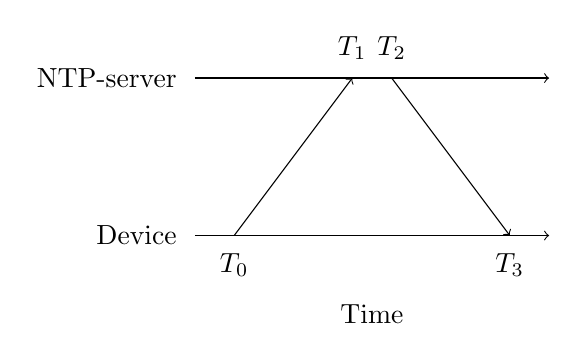
\begin{tikzpicture}[auto]
        \draw[->] (0, 0) -- (4.5, 0);
        \draw[->] (0,-2) -- (4.5,-2);

        \draw[->] (0.5, -2) -- (2, 0);
        \draw[->] (2.5, 0) -- (4.0, -2);

        \draw (2.25, -3) node {Time} node[above=3pt] {$   $};

        \draw (0,  0) node[left=3pt] {NTP-server};
        \draw (0, -2) node[left=3pt] {Device};

        \draw (0.5, -2) node[below=3pt] {$T_0$};
        \draw (4.0, -2) node[below=3pt] {$T_3$};
        \draw (2  ,  0) node[above=3pt] {$T_1$};
        \draw (2.5,  0) node[above=3pt] {$T_2$};
    \end{tikzpicture}
    \caption{The timestamps sent and received during \ac{NTP} synchronization.}
    \label{fig:ntp_packets}
\end{figure}

Here $T_0$ is the timestamp, on the device, where the request was sent, $T_1$ is the timestamp, on the \ac{NTP}-server, when the request was received.
$T_2$ is the timestamp, on the \ac{NTP}-server, when the response was sent, and $T_3$, is the timestamp, on the device, when the response was received.
Given this, one can calculate the offset, $\theta$, with the equation \ref{eq:ntp}.

\begin{equation}\label{eq:ntp}
    \theta = \frac{(t_1 - t_0)+(t_2 - t_3)}{2}
\end{equation}

When using \ac{NTP} one also have to decide on what \ac{NTP}-server to use.
We decided to use \url{0.dk.pool.ntp.org} which is a free to use \ac{NTP}-pool, and its servers are located in Denmark, furthermore we get a very low latency to them, which can improve the accuracy of the synchronization.

\subsection{Time-synchronization over WiFi Direct}
As we explained in the start of this section, we would consider it advantageous not to require our users to be connected to the Internet.
Implementing time-synchronization over WiFi Direct, independently of any third-party server on this internet would remove this requirement.

Our way of time-synchronization over WiFi Direct, uses the same methods as the method we just explained about \ac{SNTP} over the Internet, with the change that the master of the network would also act as an \ac{NTP}-server.

Implementing this requires us to add two protobufs, one for the request, and one for the response.
The request contains a single timestamp: the timestamp of the slave when it sent the request.
The response contains three timestamps: it sends the initial timestamp which it received from the slave, the timestamp for when it received it, and the timestamp for when it sends the response.
From this the slave can note the timestamp when it receives the response, and thus it has all four timestamps, and can calculate its clock offset, $\theta$, relative to the master clock.

Implementing this on the master is really simple, since it now is the master clock, the offset of it to the master clock is by definition zero.
Additionally it has to receive the requests and respond to them.
This is done by registering a callback which will be called whenever a request comes in, then record the two timestamps, build the response, and send it back.

The slave has to send the requests periodically, in order to avoid clock drift.
And like the master, it has to register a callback for when responses arrive, from which is can calculate the offset and save it.
Any part of the system which needs the offset can then ask for it, and will receive the latest recorded offset.

\subsection{Using the Synchronization in the App}
Now that we have offsets, we can therefore convert local timestamps to be synchronized with the rest of the network.
For simplicity we decided to use the offset our synchronization gave us just before sending messages over the network, and just after receiving them.
That is, when we send a message, the timestamp in it is of the master clock, and when we receive a message, it is converted to the local clock.
This is illustrated in \ref{fig:sntp_example}.\tnnote{Jeg forstår ikke helt figuren og sammenhængen mellem figuren og teksten.}
Given this setup, the offsets are $-1s925ms$ for the master relative to the \ac{NTP}-server, and $-0s937.5ms$ for the slave relative to the \ac{NTP}-server.

Say for example that we want to start playback in one second, $02s175ms$ (\ac{NTP} time), then the master would give that as the timestamp for the PlayCommand.
When the slave receives the message it will then translate the timestamp to its local time, by subtracting its offset:
$-0s937.5ms$ from the timestamp $02s175ms$: $02s175ms - (-0s937.5ms) = 3s112.5ms$.
That means that the slave should start the playback at $3s112.5ms$ on its own clock.
The master should start its playback at $02s175ms - (-1s925ms) = 4s100ms.$

\begin{figure}[bth]
    \centering
    \begin{tikzpicture}[auto, line cap=rect,line width=1pt]
        % Baggrund
        \filldraw [fill=GoogleLightBlue] (0,0) circle [radius=1cm];
        % Tick hver 3. time
        \foreach \angle in {0,90,180,270}
          \draw[line width=2pt] (0,0) -- ++(\angle:0.975cm);

        \foreach \angle in {0,90,180,270}
          \draw[line width=3pt, color=GoogleLightBlue] (0,0) -- ++(\angle:0.80cm);
        % Time viser
        %\draw[line width=1.8pt] (0,0) -- ++(150:0.5cm);
        % Minut viser
        \draw[line width=1.2pt] (0,0) -- ++(70:0.7cm);


        % Baggrund
        \filldraw [fill=GoogleAmber] (3,0) circle [radius=1cm];
        % Tick hver 3. time
        \foreach \angle in {0,90,180,270}
          \draw[line width=2pt] (3,0) -- ++(\angle:0.975cm);

        \foreach \angle in {0,90,180,270}
          \draw[line width=3pt, color=GoogleAmber] (3,0) -- ++(\angle:0.80cm);
        % Time viser
        %\draw[line width=1.8pt] (3,0) -- ++(150:0.5cm);
        % Minut viser
        \draw[line width=1.2pt] (3,0) -- ++(85:0.7cm);


        % Baggrund
        \filldraw [fill=GoogleLightGreen] (6,0) circle [radius=1cm];
        % Tick hver 3. time
        \foreach \angle in {0,90,180,270}
          \draw[line width=2pt] (6,0) -- ++(\angle:0.975cm);

        \foreach \angle in {0,90,180,270}
          \draw[line width=3pt, color=GoogleLightGreen] (6,0) -- ++(\angle:0.80cm);
        % Time viser
        %\draw[line width=1.8pt] (6,0) -- ++(150:0.5cm);
        % Minut viser
        \draw[line width=1.2pt] (6,0) -- ++(80:0.7cm);

        \node[draw, thick, fill=GoogleLightBlue]    at (0,-1.6) {Master};
        \node[]                                     at (0,-2.2) {$03s050ms$};
        \node[draw, thick, fill=GoogleAmber]        at (3,-1.6) {NTP-server};
        \node[]                                     at (3,-2.2) {$01s175ms$};
        \node[draw, thick, fill=GoogleLightGreen]   at (6,-1.6) {Slave};
        \node[]                                     at (6,-2.2) {$02s250ms$};
    \end{tikzpicture}
    \caption{Example of \ac{SNTP} over the Internet in action, only the second hand is shown.}
    \label{fig:sntp_example}
\end{figure}

This approach has some advantages and disadvantages\tnnote{Pros and cons table}, the biggest advantage is simplicity, it allows us to only think about time synchronization in one place, and not in the player itself.
However the disadvantage is that the longer we buffer data, the more outdated it gets.


% Hvor ofte skal vi synkronisere!?!

% eksempel på begge ?!?